\documentclass{cmspaper}

\usepackage{graphicx}% Include figure files

\def\etmiss{\big\slash\hspace{-1.6ex}{E_T}}

\begin{document}

%==============================================================================
% title page for few authors

\begin{titlepage}

  % select one of the following and type in the proper number:
  \cmsnote{2005/000}
%  \internalnote{2005/000}
%  \conferencereport{2005/000}
%  \cmsan{2005/000}
%  \cmsdtnote{2005/000}
%  \cmspas{2005/000}
   \date{1 April 2005}

  \title{CMS Paper Template - LaTeX version}

  \begin{Authlist}
    A.~Author, B.~Author, C.~Author\Aref{a}
       \Instfoot{cern}{CERN, Geneva, Switzerland}
    D.~Author, E.~Author\Aref{b}, F.~Author
       \Instfoot{ieph}{Institute of Experimental Physics, Hepcity, Wonderland}
  \end{Authlist}

% if needed, use the following:
%\collaboration{Flying Saucers Investigation Group}
%\collaboration{CMS collaboration}

  \Anotfoot{a}{On leave from prison}
  \Anotfoot{b}{Now at the Moon}

  \begin{abstract}
    This is a template written in LaTeX,
    processed with {\it cmspaper.cls} document class.
    It is based on the {\it cernart.cls} and {\it articlet.cls} classes.
    The above information, Title and Abstract, should be readable on any 
    computer and should be searchable on the information server. 
    Therefore if the abstract or the title of your note contains Greek 
    characters and mathematical symbols, please send to the CMS secretariat 
    alternative versions which do not contain such characters.
  \end{abstract} 

% if needed, use the following:
%\conference{Presented at {\it Physics Rumours}, Coconut Island, April 1, 2005}
%\submitted{Submitted to {\it Physics Rumours}}
%\note{Preliminary version}
  
\end{titlepage}

\setcounter{page}{2}%JPP

%==============================================================================
% title page for many authors
%
%\begin{titlepage}
%  \internalnote{2005/000}
%  \title{CMS Technical Note Template}
%
%  \begin{Authlist}
%    A.~Author\Iref{cern}, B.~Author\Iref{cern}, C.~Author\IAref{cern}{a},
%    D.~Author\IIref{cern}{ieph}, E.~Author\IIAref{cern}{ieph}{b},
%    F.~Author\Iref{ieph}
%  \end{Authlist}
%
%  \Instfoot{cern}{CERN, Geneva, Switzerland}
%  \Instfoot{ieph}{Institute of Experimental Physics, Hepcity, Wonderland}
%  \Anotfoot{a}{On leave from prison}
%  \Anotfoot{b}{Now at the Moon}
%
%  \begin{abstract}
%    This is a template of a CMS paper, written in LaTeX,
%    processed with {\it cmspaper.sty} style.
%    It is based on the {\it cernart.sty} and {\it articlet.sty} styles.
%    There are two versions of the title page.
%    The current one is designed for many authors.
%    The one on the previous page is for few authors.
%    Just delete the one which you do not need.
%  \end{abstract} 
%  
%\end{titlepage}
%
%==============================================================================

\section{Introduction}

    There are three kind of CMS papers: ``CMS Note'', 
    ``CMS Internal Note'' and ``CMS Conference Report''.
    They differ only in the header of the first page,
    which includes an eps figure different for each kind.
    One of the following commands must be selected,
    where \verb$yyyy$ is the current year
    and \verb$xxx$ is the document number allocated by the CMS secretariat:
{\small \begin{verbatim}
  \cmsnote{yyyy-xxx}
  \internalnote{yyyy-xxx}
  \conferencereport{yyyy-xxx}
\end{verbatim} }
    
Apart from the title and authors some supplementary information can be given
on the first page:
{\small \begin{verbatim}
  \collaboration{Physics Analysis Group}
  \conference{Presented at {\em Hard Collisions}, Coconut Island, May 2005}
  \submitted{Submitted to {\em Physics Rumours}}
  \note{Preliminary version}
\end{verbatim} }

\section{Data Samples and Event Selection}

Trigger, DataSample, Good Run List. Mention separate 900 GeV and 2.36
TeV. 

\subsection{Vertex selection}
Show vertex distributions, discuss some group's selections on vertex.

\subsection{Removal of scraping events}
This is an example of subsection

\subsection{HCAL anomalous noise}

This is an example of subsection

\subsection{ECAL anomalous noise}

This is an example of subsection

\begin{2figures}{hbtp}
  \resizebox{8cm}{!}{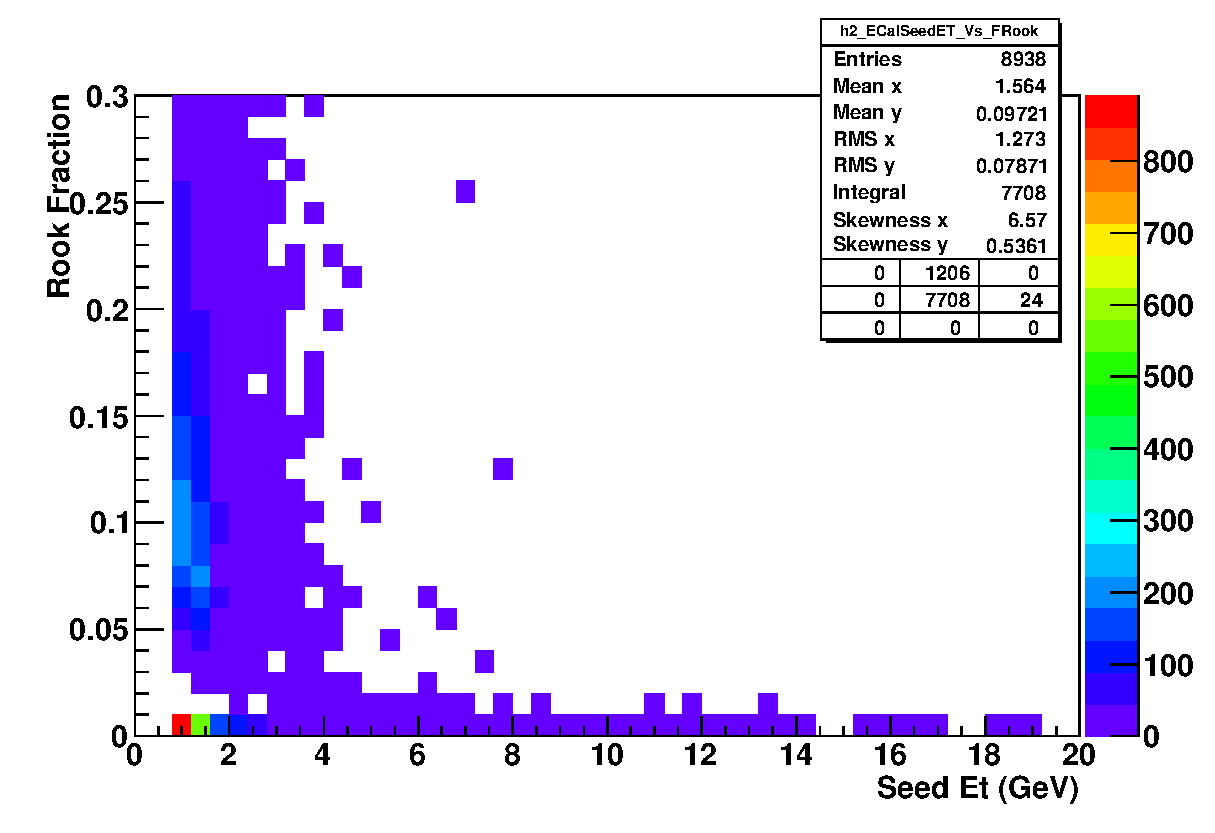
\includegraphics{plots_ecalnoise/SeedET_Frook_DATA900GeV.eps}} &
  \resizebox{8cm}{!}{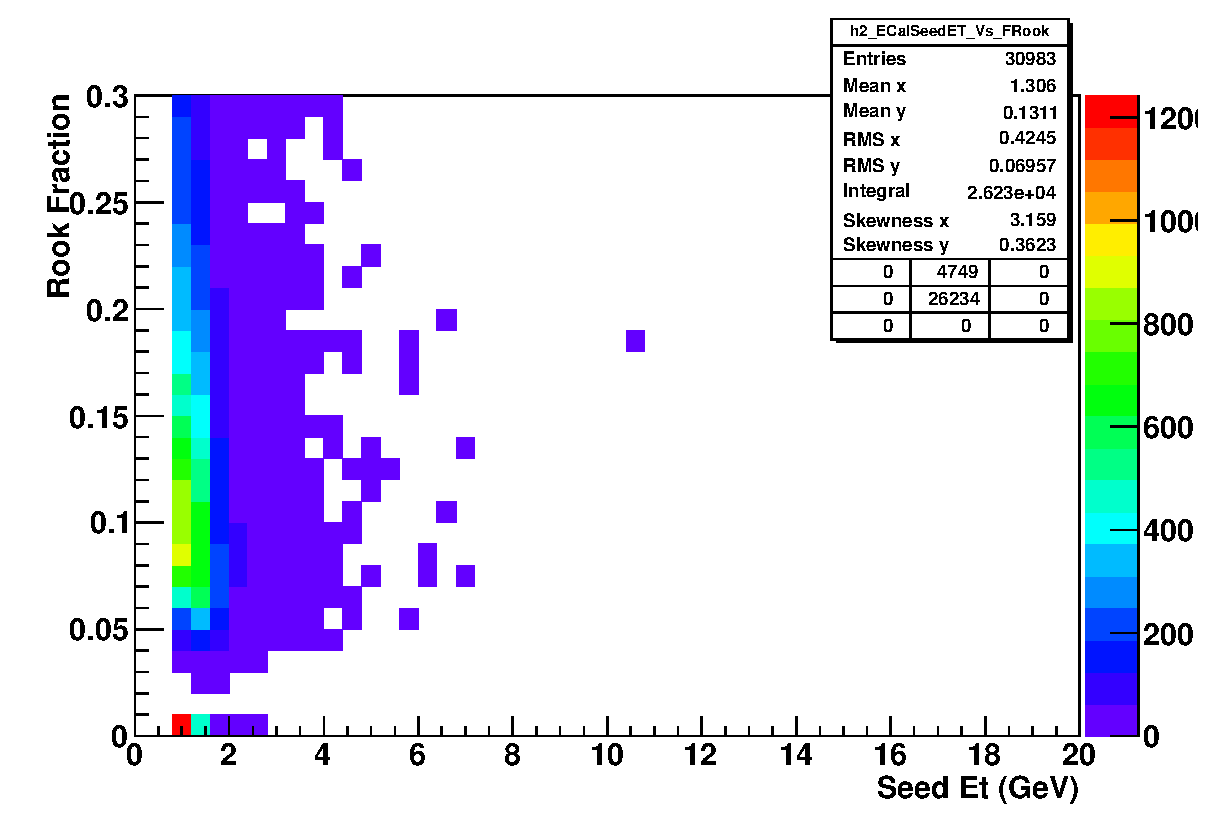
\includegraphics{plots_ecalnoise/SeedET_Frook_MC900GeV.eps}} \\
\caption{900 GeV Data Vs MC}
 \label{fig:ecal_noise_1}
\end{2figures}

Add cut efficiency table HERE.

\begin{table}[htbp]
 \label{tab:HEEPselection}
 \begin{center}
   \begin{tabular}{|lcc|lcc|} \hline
     \multicolumn{3}{|c|}{ID Variables} & \multicolumn{3}{|c|}{Isolation Variables} \\
     Variable & Barrel & Endcap & Variable & Barrel & Endcap  \\ \hline
     $H/E$  & $<0.05$ & $<0.1$ & $N_T$  & $<4$ & $<4$ \\ \hline
     $\sigma_{\eta\eta}$  & $<0.011$ & $<0.0275$ & Track iso (GeV) & $<7.5$ & $<15$ \\ \hline
     $|\Delta\eta^{trk-SC}|$ & $<0.005$ & $<0.007$ & EM iso (GeV) & $<6+0.01*E_{t}$ & $<6+0.01*E_{t}$ \\ \hline
     $|\Delta\phi^{trk-SC}|$ & $<0.09$ & $<0.09$ & HAD iso (GeV) & $<4+0.005*E_{t}$ & $<4+0.005*E_{t}$ \\ \hline
   \end{tabular}
 \caption{\small \sl HEEP electron ID and isolation criteria.
   Reconstructed electrons are associated to the
   barrel (endcaps) if $|\eta|<1.442$ ($1.560<|\eta|<2.5$).}
 \end{center}
\end{table}



\subsection{Effect of noise removal}
Here we put the $\etmiss$ distribution with base selection, after HCAL/ECAL
noise removal.

\section{$\etmiss$ stability over 2009 data-taking period}

This is an example of subsection

\section{Calorimeter Noise simulation}
rechits from Dinko

\section{Data to Monte Carlo comparisons at $\sqrt{s}=900$ GeV in
  Minimum Bias events}


\subsection{Basic $\etmiss$-related distributions.}
$\etmiss$ plots, Sumet plots, in EB/EE etc.

\subsection{$\etmiss$ resolution.}
Dinko's plots of MET resolution comparison. Also fit of MET resolution.

\subsection{$\etmiss$ and SumET dependence on $\eta$}
put here plots of MET VS etaring

\section{Data to Monte Carlo comparisons at $\sqrt{s}=2.36$ TeV in
  Minimum Bias events}


\subsection{Basic $\etmiss$-related distributions.}
$\etmiss$ plots, Sumet plots, in EB/EE etc.

\subsection{$\etmiss$ resolution.}
Dinko's plots of MET resolution comparison. Also fit of MET resolution.

\subsection{$\etmiss$ and SumET dependence on $\eta$}
put here plots of MET VS etaring

\section{Data to Monte Carlo comparisons at $\sqrt{s}=900$ GeV in di-jet events} 

\section{Data to Monte Carlo comparisons at $\sqrt{s}=2.36$ TeV in di-jet events} 


\section{Summary} 


\begin{tabular}{|l|ccc|} \hline
         LaTeX name & roman & sansserif & typewriter \\
         PostScript name & Times & Helvetica & Courrier \\ \hline
      \end{tabular}

 \begin{table}[htb]
    \caption{Page layout for A4 and US letter formats.}
    \label{tab:page_layout}
    \begin{center}
      \begin{tabular}{|l|ccccc|ccccc|} \hline
               & \multicolumn{5}{c|}{mm} & \multicolumn{5}{c|}{inches} \\ 
        margin & left & right & top & bottom & foot &
                 left & right & top & bottom & foot \\ \hline
        A4 & 25 & 25 & 20 & 34 & 28 & 1.0 & 1.0 & 0.8 & 1.3 & 0.9 \\
        US letter   & 25 & 31 & 20 & 16 & 10 & 1.0 & 1.2 & 0.8 & 0.6 & 0.4 \\ \hline
      \end{tabular}
    \end{center}
  \end{table}

\begin{2figures}{hbtp}
  \resizebox{\linewidth}{0.5\linewidth}{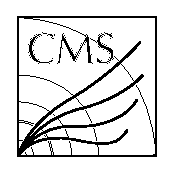
\includegraphics{cmslogo.eps}} &
  \resizebox{\linewidth}{0.5\linewidth}{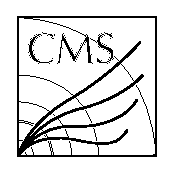
\includegraphics{cmslogo.eps}} \\
 \caption{The left figure}
  \label{fig:ex3} &
  \caption{The right figure}
  \label{fig:ex4} \\
\end{2figures}

\section{Reference example}

References should be placed at the end of the note 
(see example \cite{NOTE000}).

\begin{thebibliography}{9}
  \bibitem {NOTE000} {\bf CMS Note 2005/000},
    X.Somebody et al.,
    {\em "CMS Note Template"}.
\end{thebibliography}


\end{document}
